\chapter{Анализ предметной области}
\label{cha:analysis}
%
% % В начале раздела  можно напомнить его цель
%

%\textbf{//КОММЕНТАРИЙ:
%Формулировать задачу обязательно до обзора системы? Если знать архитектуру системы, тогда понятно как такие требования получаются...}

\section{Формулировка задачи}
В данной главе будет рассмотрена система AEM и сформулированы формальные требования на основе первоначальных требований и возможностей системы.

Adobe Experience Manager — система управления контентом, осуществляющая хранение, обработку и доставку различных видов контента в масштабах предприятия. Система предназначена для крупных компаний, имеющих потребности в управление быстро меняющимся контентом, это могут быть как и внутренние корпоративные порталы так и порталы для внешних пользователей. Созданный контент публикуется на отдельных серверах, оптимизированных для быстрого и надежного чтения хранимых ресурсов.

Основные пользователи системы:
\begin{enumerate}
\item Авторы контента или контент-менеджеры - отвечают за наполнения сайтов контентом.
\item Администратор - отвечает за развитие, поддержку работоспособности и безопасности системы.
\item Разработчик - Разработчики работающие с системой занимаются разработкой новых компонентов, шаблонов, и функционала системы.
\item Внешние пользователи - имеют доступ к контенту созданному авторами контента и расположенному на экземплярах публикации.
\end{enumerate}

В компаниях использующих AEM может быть развернуто множество так называемых Лэндскейпов - Наборов элементов аппаратного обеспечения, программного обеспечения и средств, расположенных в определенной конфигурации. Лэндскейпы включают в себя различные наборы серверов в том числе с развернутыми на них AEM средами содержащими экземпляры авторов, публикации и диспетчеры (Приложение A рис.~\ref{fig:complexDeploy}). В крупных компаниях может быть развернуто множество таких сред представляющих из себя самостоятельные порталы или сайты со своим контентом. Такие порталы или сайты могут содержать скрытый контент, доступный только авторизованным внешним пользователям. Как правило, в таких компаниях внешние пользователи имеют один аккаунт для всех систем этой компании т.е применяется технология единого входа рис.~\ref{fig:companyDiagramm}.

\begin{figure}[h]
  \centering
  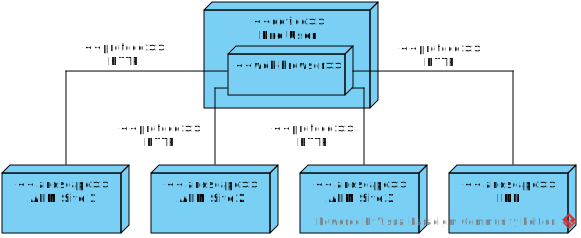
\includegraphics[width=\textwidth]{inc/svg/companyDiagramm}
  \caption{Диаграмма развертывания Лэндскейпов в компании}
  \label{fig:companyDiagramm}
\end{figure}

Несмотря на то что система AEM имеет богатый набор возможностей для авторов контента и администраторов системы, она не имеет встроенных функций для работы с внешними пользователями системы, а именно отсутствует управление авторизацией и контроль доступа для внешних пользователей системы.

Исходя из вышеописанных пунктов возникла необходимость доработки системы с целью реализации взаимодействия с развернутой в компании технологией единого входа и управления авторизацией внешних пользователей на сайтах и порталах компании использующих AEM. Исходные данные и требования полученные от компании: 
\begin{itemize} 
\item В компании развернут поставщик учетных записей, работающий по протоколу SAML.
\item В компании имеется три портала работающих на основе системы AEM.
\item Разрабатываемое решение должно легко внедрятся во все существующие и будущие порталы на базе AEM.
\item Разрабатываемое решение должно поддерживать технологии единого входа и  выхода.
\item Должна быть возможность использовать различные SAMl привязки, которые должны быть настраиваемыми в каждом приложение.
\item Данные пользователей не должны хранится в хранилище данных системы AEM. Должны хранится только данные сессии, которая имеет короткое время жизни.
\end{itemize}
% Обратите внимание, что включается не ../dia/..., а inc/dia/...
% В Makefile есть соответствующее правило для inc/dia/*.pdf, которое
% берет исходные файлы из ../dia в этом случае.

%\begin{figure}
%  \centering
%  \includegraphics[width=\textwidth]{inc/dia/rpz-idef0}
%  \caption{Рисунок}
%  \label{fig:fig01}
%\end{figure}
%
%В \cite{Pup09} указано, что...
%
%Кстати, про картинки. Во-первых, для фигур следует использовать \texttt{[ht]}. Если и после этого картинки вставляются <<не по ГОСТ>>, т.е. слишком далеко от места ссылки,~--- значит у вас в РПЗ \textbf{слишком мало текста}! Хотя и ужасный параметр \texttt{!ht} у окружения \texttt{figure} тоже никто не отменял, только при его использовании документ получается страшный, как в ворде, поэтому просьба так не делать по возможности.

\section{Обзор системы и существующих компонентов}

AEM – система построенная с использованием технологии Java. В основе системы лежит фреймворк OSGI. Фреймворк имеет свой контекст, в который и устанавливаются все модули, они взаимодействуют между собой по средствам сервисов зарегистрированных в регистре сервисов рис.~\ref{fig:servicePattern}. Под динамической системой понимается возможность устанавливать, удалять и обновлять модули без перезапуска системы.

\begin{figure}[h]
  \centering
  \includegraphics[width=\textwidth]{inc/svg/servicePattern}
  \caption{Диаграмма архитектуры OSGI}
  \label{fig:servicePattern}
\end{figure}

\subsection{Архитектура AEM}
Основу AEM составляют набор модулей, которые можно условно выделить в 4 компоненты:
\begin{enumerate}
\item Java content repository – один из типов объектной базы данных, созданных для хранения и извлечения иерархических данных. Данные в JCR представляют из собой дерево, состоящее из узлов с ассоциированными с ними свойствами. Эти свойства и являются хранимыми данными, и могут хранить строки, числа или основные примитивные типы данных, а так-же двоичные данные, изображения и.т.д. 
\item Apache Sling – веб-фреймворк построенный по архитектуре REST, отвечающий за доставку контента в контент-ориентированных приложениях с использованием JCR.
\item AEM модули – набор бандлов реализованных компанией Adobe с использованием вышеупомянутых технологий.
\item Пользовательские модули – модули, разрабатываемые разработчиками, и расширяющие функционал системы.
\end{enumerate}

\begin{figure}[h]
  \centering
  \includegraphics[width=\textwidth]{inc/dia/osgi}
  \caption{Архитектура AEM}
  \label{fig:fig02}
\end{figure}

%\textbf{//Комментарий: Если дальше буду говорить про какие-то фишки системы которые проверяю, т.е РЕПЛИКАЦИЯ, Режимы запуска, Жизненный цикл компонентов, то их тоже нужно тут указать?}
%Выделить какой-то абзац под описание ключевых фишек(компонентов) AEM
\subsection{Обзор SAML модулей системы}
В системе имеется SAML модуль - "Adobe Granite - SAML 2.0 Authentication Handler" \cite{web:aemSaml}, предназначенный для интеграции с поставщиком учетных записей. Данный модуль имеет конфигурацию представленную на рис.~\ref{fig:defaultHandlerConfig1} и рис.~\ref{fig:defaultHandlerConfig2}. Рассмотрим подробнее следующие параметры конфигурации:
\begin{itemize}
\item path - путь до контента по которому будет вызван данный обработчик.
\item idpUrl - URL поставщика учетных записей который обрабатывает запросы на авторизацию.
\item idpCertAlias - имя сертификата IdP.
\item serviceProviderEntityId - имя поставщика сервиса сохраненное в IdP.
\item keyStorePassword - пароль от хранилища сертификатов.
\item defaultRedirectUrl - URL на который пользователь будет перенаправлен после успешной авторизации.
\item useEncryption - шифровать сообщения с помощью сертификата из хранилища.
\item createUser - создавать пользователя внутри системы AEM если он не был создан ранее.
\item defaultGroups - группа в которую будет добавлен пользователь при создании.
\item synchronizeAttributes - синхронизировать атрибуты из ответа SAML с атрибутами созданного пользователя.
\item handleLogout - обрабатывать запросы на выход из приложения.
\item logoutUrl - URL выхода, по которому будет вызван данный обработчик.
\end{itemize}

Данный обработчик либо создает пользователя в системе при первой авторизации если выбран параметр "createUser" или требует уже созданного пользователя. Также требуется назначить данных пользователей в соответствующие группы, а также страницам должны быть назначены эти группы. 

Вывод: Несмотря на то что данный подход реализует технологию единого входа он использует хранилище на экземплярах публикации для хранения пользователей, что требует синхронизации между всеми экземплярами публикации и разработки дополнительного функционала для связи атрибутов пользователя с IdP с атрибутами  хранящимся в системе. Необходимость хранить данные пользователей в системе противоречит требованиям и может быть использовано только для экземпляров автора. Также конфигурация реализует только один тип SAML привязки - "HTTP POST binding". Существующий модуль не может удовлетворить поставленные требования, в связи с чем было принято решение разработать новый модуль который будет выступать в роли полноценного поставщика сервиса.

\section{Формальные требования}
Данный раздел уточняет и формирует требования к разрабатываемому модулю.

\subsection{Функциональные требования}
Разрабатываемый модуль должен удовлетворять следующим требованиям:
\begin{itemize}
\item Получает запросы на авторизацию, формирует SAML запрос авторизации и  переправляет пользователя на IdP.
\item Получает запросы на выход из системы формирует SAML запрос выхода из системы и переправляет пользователя на IdP.
\item Получает SAML ответ авторизации, обрабатывает его и при успешном ответе сохраняет cookie пользователя.
\item Получает SAML ответ выхода, обрабатывает его и при успешном ответе удаляет сохраненные cookie пользователя.
\item Получает SAML запрос выхода, обрабатывает его, удаляет сохраненные cookie пользователя и формирует ответ для IdP.
\item Все сообщения должны быть подписаны с использованием сертификата хранящегося в Java Keystore.
\item Должен иметь набор конфигураций.
\end{itemize}

\subsection{Требования к конфигурации}
Модуль должен содержать два вида конфигурации:
\begin{itemize}
\item Base SAML Configuration - содержит единые параметры для всех поставщиков сервиса в системе.
\item Service Provider Configuration - позволяет задать в одной системе несколько поставщиков сервиса со своими параметрами. 
\end{itemize}

Требуемые параметры конфигурации "Base SAML Configuration":
\begin{itemize}
\item Cookie expiration - время жизни cookie в секундах.
\item IdP metadata URI - URL по которому доступны метаданные IdP.
\item JVM Keystore location - путь до Java хранилища ключей.
\item JVM Keystore password - пароль от Java хранилища ключей.
\item SAML Binding type - тип привязки SAML.
\end{itemize}

Требуемые параметры конфигурации "Service Provider Configuration":
\begin{itemize}
\item Service Provider ID - идентификатор поставщика услуг.
\item Service Provider Name - имя поставщика услуг.
\item Certificate Alias - имя сертификата в Java хранилище ключей.
\item Certificate Password - пароль сертификата в Java хранилище ключей.
\item Assertion Consumer Service URI - URL который обрабатывает утверждения полученные от IdP.
\item Cookie Name - имя cookie которые сохраняются при авторизации.
\item Redirect Landing Page URL - URL если необходимо перенаправление пользователя после авторизации.
\item Error Redirect URL - URL если обрабатывающий ошибку произошедшую в процессе авторизации.
\end{itemize}

\section{Заключение}
В данной главе был произведен обзор системы и рассмотрены сценарии при которых возникает необходимость разработки нового модуля для управления авторизацией в системе AEM с использованием SAML. Встроенные механизмы для реализации авторизации с помощью SAML не соответствуют всем требованиям заказчика. Было принято решение разработать новый модуль который можно будет использовать во всех проектах заказчика использующих AEM.


%%% Local Variables:
%%% mode: latex
%%% TeX-master: "rpz"
%%% End:
